\documentclass[12pt,a4paper]{article}
\usepackage{amsmath}
\usepackage{amssymb}
\usepackage{graphicx}
\usepackage{hyperref}
\usepackage{natbib}
\usepackage{url}
\usepackage{xcolor}
\usepackage{booktabs}
\usepackage{caption}
\usepackage{subcaption}
\usepackage{setspace}
\usepackage{geometry}
\usepackage{float}
\usepackage{enumitem}
\usepackage{fancyhdr}
\usepackage{microtype}
\usepackage[T1]{fontenc}
\usepackage{lmodern}
\usepackage{pdflscape}

% Set headheight to fix fancyhdr warning
\setlength{\headheight}{14.5pt}

% Set page geometry
\geometry{
 a4paper,
 total={170mm,257mm},
 left=20mm,
 right=20mm,
 top=20mm,
 bottom=20mm,
}

% Configure section heading formatting
\usepackage{titlesec}
\titleformat{\section}{\large\bfseries}{\thesection}{1em}{}
\titleformat{\subsection}{\normalsize\bfseries}{\thesubsection}{1em}{}

% Configure fancy headers
\pagestyle{fancy}
\fancyhf{}
\fancyhead[L]{Supplementary Material - Enhanced Bioreactor Synthesis}
\fancyhead[R]{\thepage}
\renewcommand{\headrulewidth}{0.4pt}

% Configure hyperref
\hypersetup{
    colorlinks=true,
    linkcolor=blue,
    filecolor=magenta,
    urlcolor=blue,
    citecolor=blue,
    pdftitle={Supplementary Material - Enhancing Nitrate Removal in Denitrifying Woodchip Bioreactors},
    pdfauthor={Reza Moghaddam and Laura E. Christianson},
}

% Configure figure and table placement
\renewcommand{\topfraction}{0.85}
\renewcommand{\bottomfraction}{0.85}
\renewcommand{\textfraction}{0.1}
\renewcommand{\floatpagefraction}{0.75}

\title{Supplementary Material\\
\large Enhancing Nitrate Removal in Denitrifying Woodchip Bioreactors: A Comprehensive Analysis of Enhancement Strategies and Environmental Trade-offs}

\author{Reza Moghaddam\textsuperscript{1} and Laura E. Christianson\textsuperscript{2}}
\date{\today}

\begin{document}

\maketitle

\begin{center}
\footnotesize
\textsuperscript{1}Earth Sciences New Zealand\\
\textsuperscript{2}Research Associate Professor, Department of Crop Sciences, University of Illinois at Urbana-Champaign\\
S-322 Turner Hall, Urbana, IL 61801, USA\\
Corresponding author: reza.moghaddam@niwa.co.nz
\end{center}

\section{Introduction}

This supplementary material provides advanced synthesis visualizations and meta-analytical perspectives that complement the main manuscript. The figures presented here offer comprehensive frameworks for understanding enhancement pathways, cross-cutting performance patterns, and integrated technology assessment approaches for denitrifying woodchip bioreactor systems.

\section{Advanced Synthesis Figures}

\subsection{Comprehensive Enhancement Pathways Framework}

Figure S1 presents a comprehensive synthesis of enhancement strategies and their interconnected relationships within the bioreactor technology landscape. This four-panel visualization provides a holistic view of enhancement approaches, environmental trade-offs, temporal development patterns, and integration frameworks that collectively inform optimal system design and implementation strategies.

\begin{figure}[H]
\centering
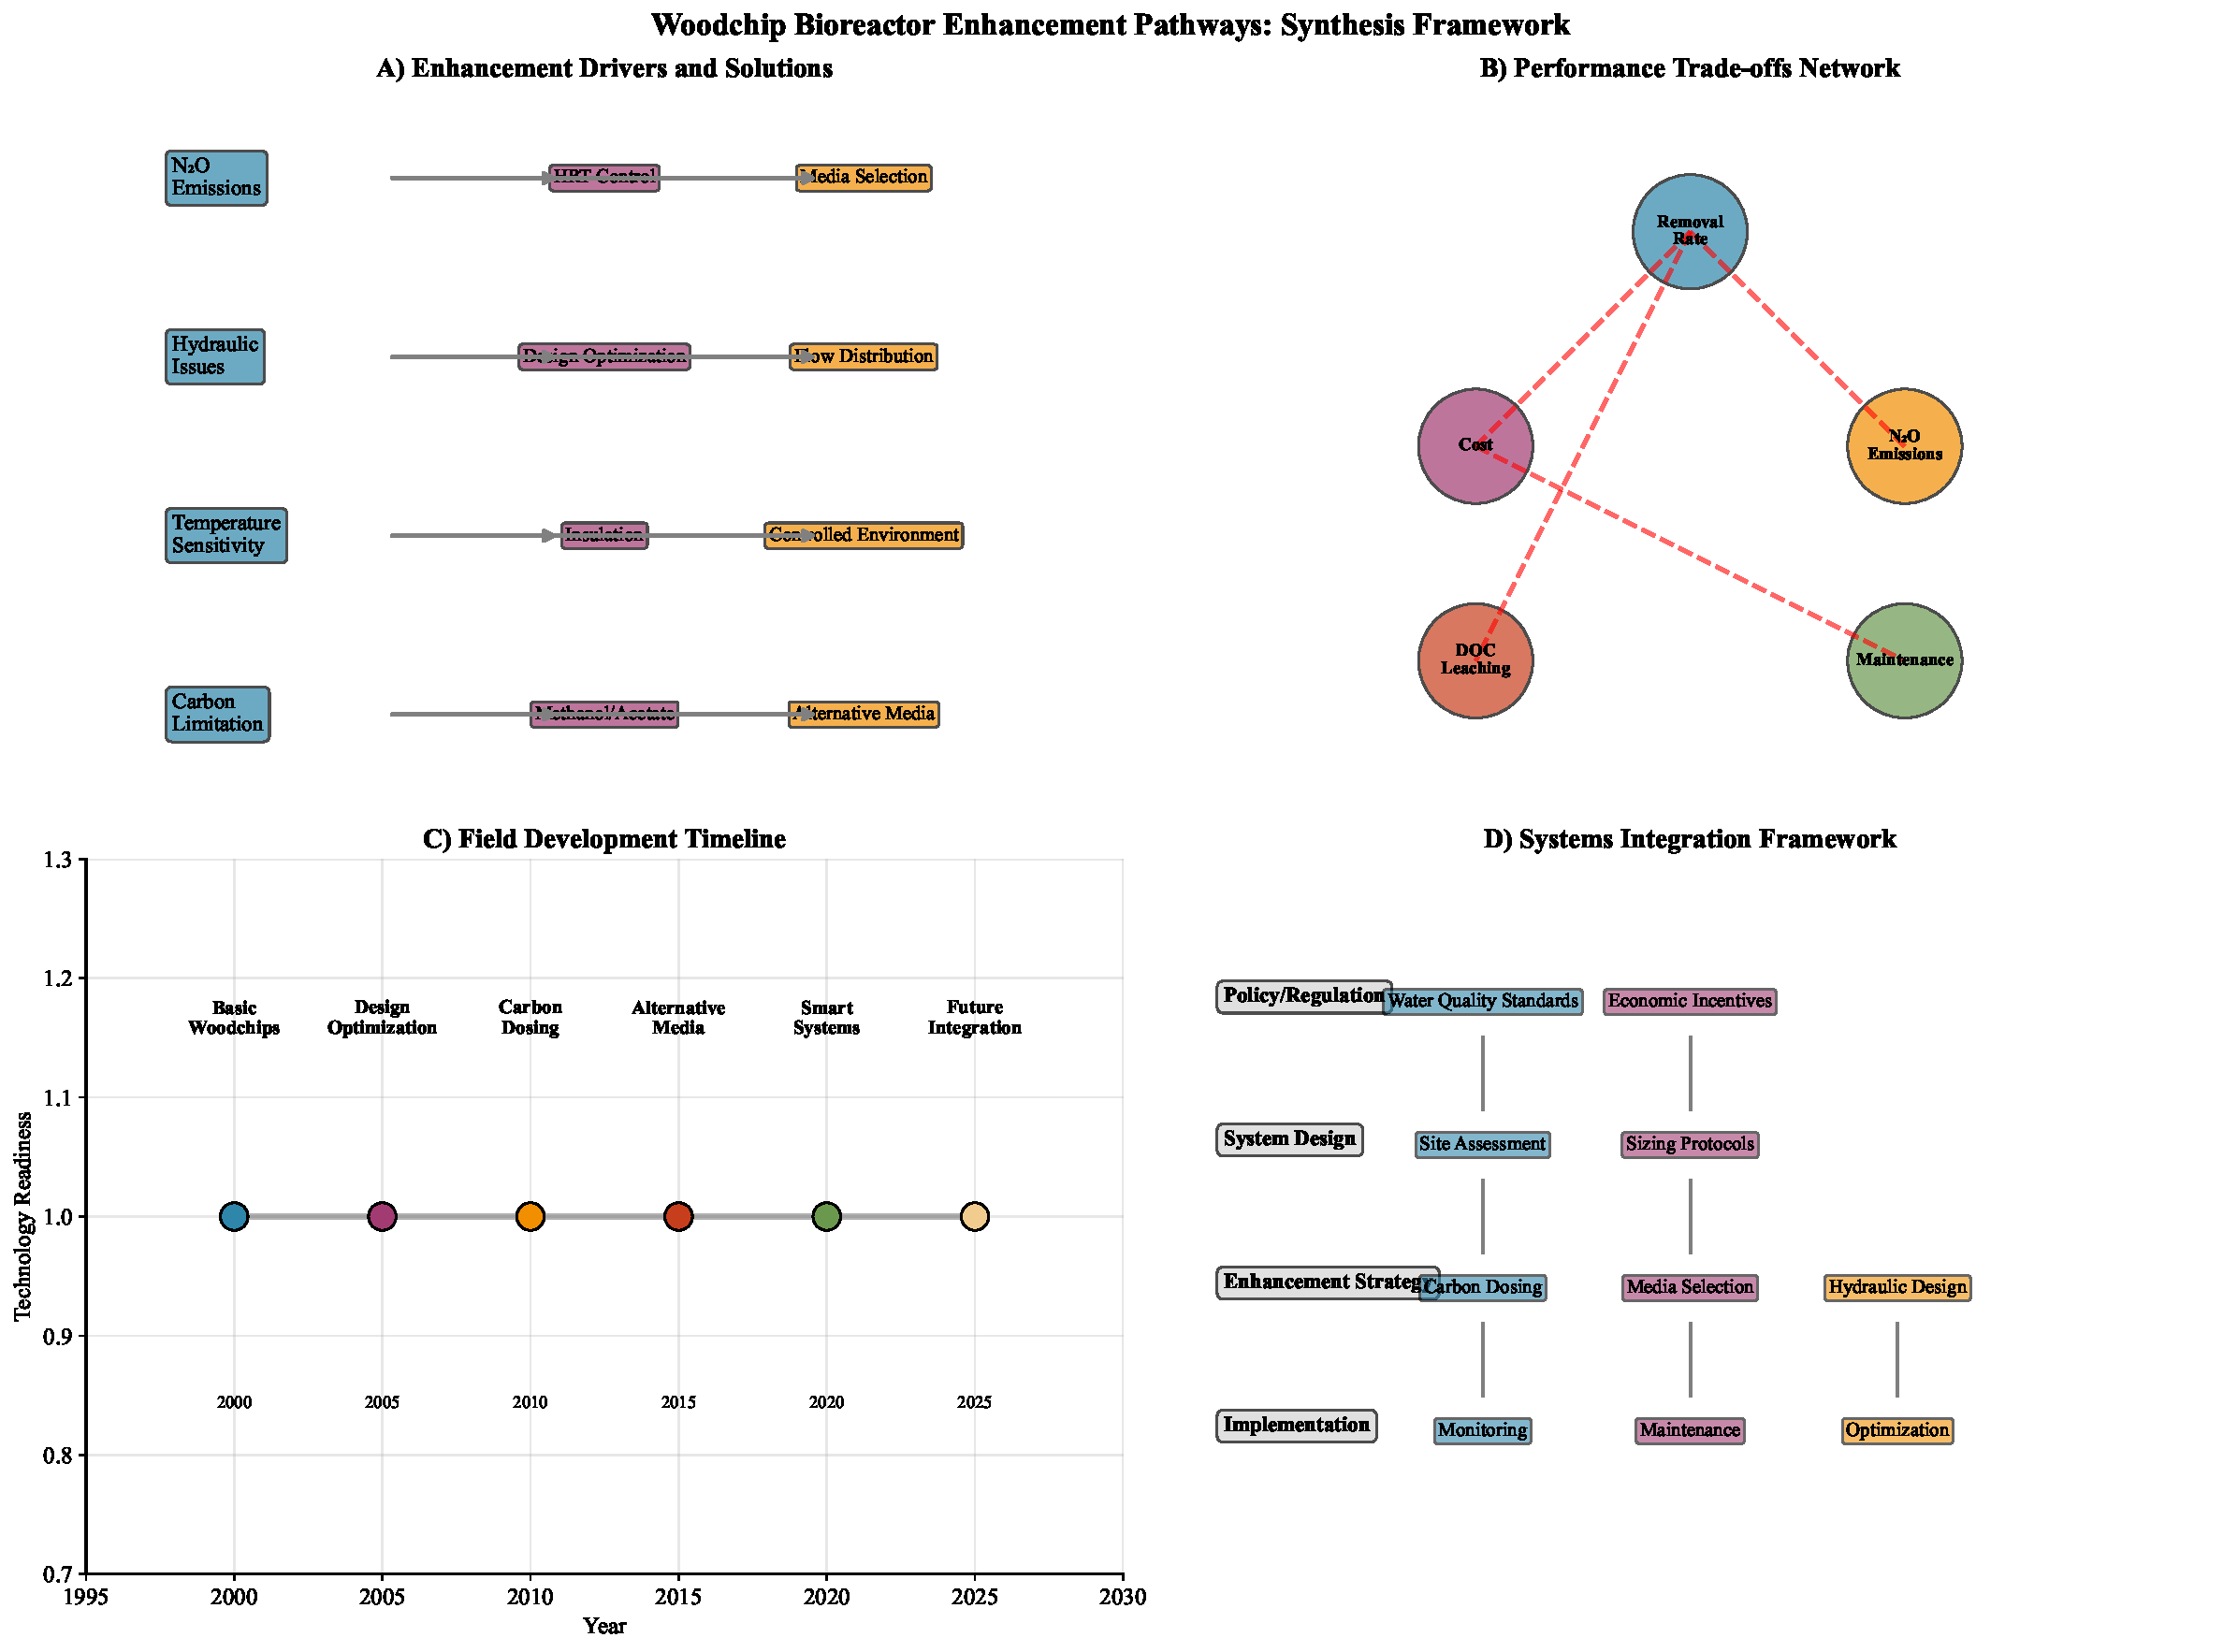
\includegraphics[width=1.0\textwidth]{fig_synthesis_enhancement_pathways}
\caption{\textbf{Woodchip bioreactor enhancement pathways synthesis framework.} 
\textbf{Panel A:} Enhancement drivers and solutions network showing four main limitation categories (Carbon Limitation, Temperature Sensitivity, Hydraulic Issues, N$_2$O Emissions) with their corresponding solution pathways. Carbon limitation is addressed through methanol/acetate dosing or alternative media; temperature sensitivity through insulation or controlled environments; hydraulic issues through design optimization and flow distribution; and N$_2$O emissions through hydraulic retention time (HRT) control and media selection.
\textbf{Panel B:} Performance trade-offs network displaying interconnected relationships between removal rate (central blue node) and key trade-off factors including cost, N$_2$O emissions, DOC leaching, and maintenance requirements. Red dashed lines indicate negative trade-offs where improving one parameter may compromise another.
\textbf{Panel C:} Field development timeline showing technology readiness evolution from 2000-2030, with distinct phases: Basic Woodchips (2000), Design Optimization (2005), Carbon Dosing (2010), Alternative Media (2015), Smart Systems (2020), and projected Future Integration (2025). Technology readiness scale ranges from 0.7 to 1.3.
\textbf{Panel D:} Systems integration framework hierarchy showing four implementation levels: Policy/Regulation (water quality standards, economic incentives), System Design (site assessment, sizing protocols), Enhancement Strategy (carbon dosing, media selection, hydraulic design), and Implementation (monitoring, maintenance, optimization).}
\label{fig:synthesis_pathways}
\end{figure}

\subsubsection{Interpretation and Implications}

The enhancement pathways framework reveals several critical insights for technology development and implementation:

\textbf{Problem-Solution Mapping:} Panel A demonstrates that each major limitation category has specific solution pathways. Carbon limitation (the most fundamental constraint) can be addressed through either chemical supplementation (methanol/acetate) or biological enhancement (alternative media). Temperature sensitivity requires physical solutions (insulation, controlled environments), while hydraulic issues demand engineering optimization (design improvements, flow distribution). N$_2$O emissions are controlled through operational parameters (HRT management) and material selection.

\textbf{Central Role of Removal Rate:} Panel B illustrates that removal rate serves as the central performance metric with trade-off relationships to all other factors. The network structure shows that achieving higher removal rates typically involves trade-offs with cost, maintenance requirements, and potential for N$_2$O emissions or DOC leaching. This emphasizes the need for balanced optimization rather than single-objective maximization.

\textbf{Technology Maturation Timeline:} Panel C shows a clear evolution in technology readiness over 30 years, with each major advancement occurring approximately every 5 years. The progression from basic woodchips (1.0 readiness baseline) through design optimization, carbon dosing, alternative media, to smart systems demonstrates systematic field advancement. Future integration (2025+) suggests convergence toward optimized multi-strategy approaches.

\textbf{Implementation Hierarchy:} Panel D provides a practical implementation framework with four distinct levels requiring coordination. Policy/regulation sets the boundary conditions, system design establishes technical parameters, enhancement strategy selection determines operational approach, and implementation ensures effective deployment. Success requires alignment across all levels.

\subsection{Meta-Analysis Performance Synthesis}

Figure S2 presents a meta-analytical synthesis of performance data across enhancement strategies, providing quantitative comparison frameworks and uncertainty analysis that inform evidence-based technology selection and performance prediction.

\begin{figure}[H]
\centering
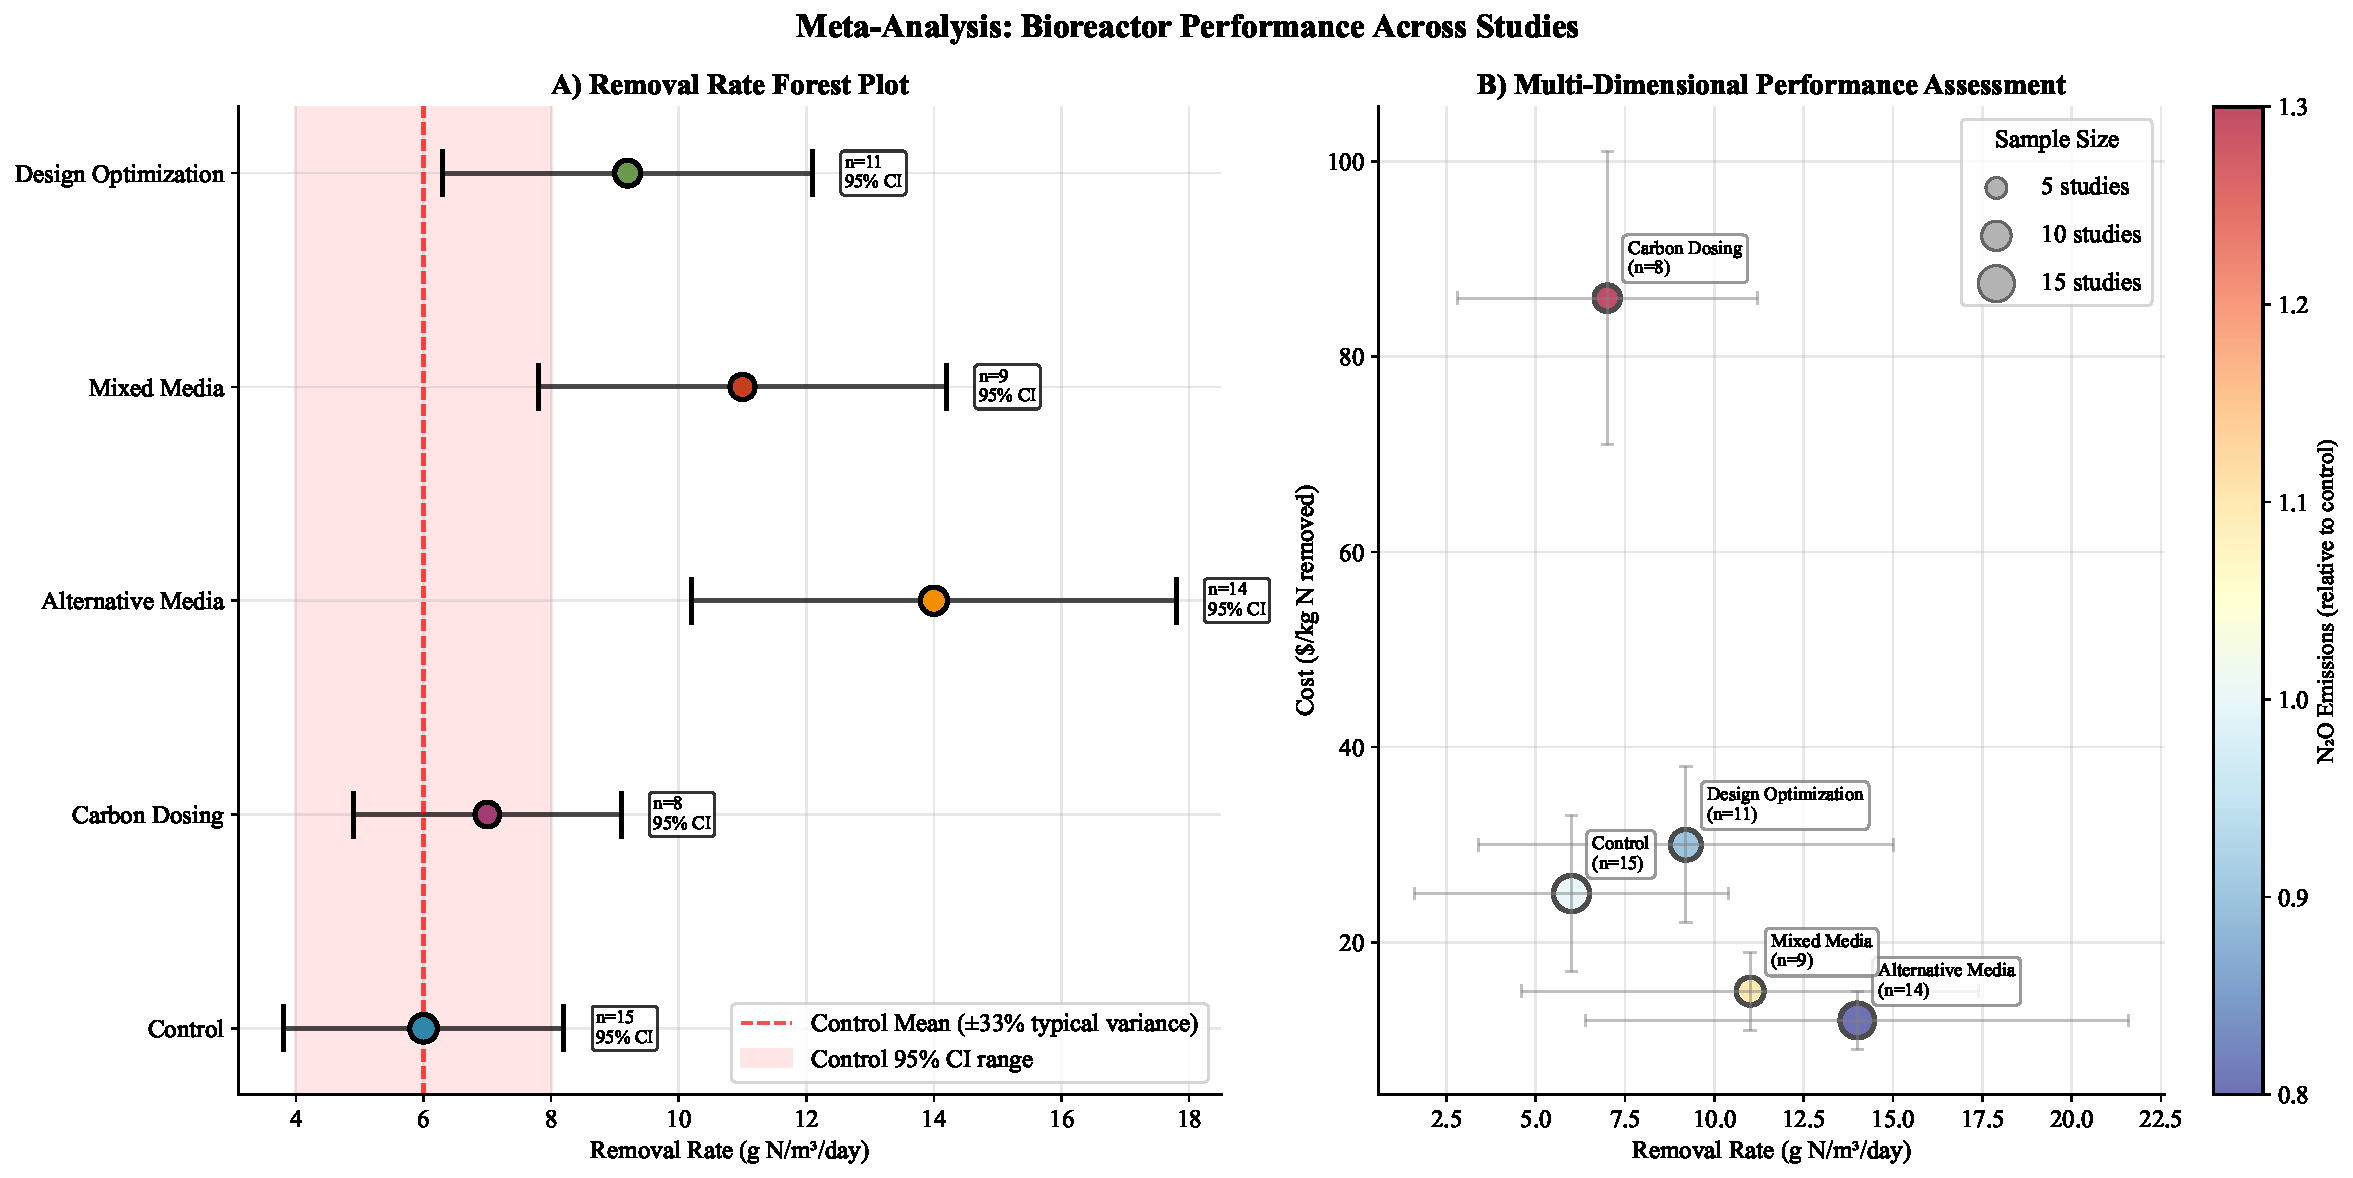
\includegraphics[width=1.0\textwidth]{fig_meta_analysis_performance}
\caption{\textbf{Meta-analysis of bioreactor performance across enhancement strategies.}
\textbf{Panel A:} Forest plot showing nitrate removal rate comparisons across five enhancement categories with 95\% confidence intervals. Control baseline (red dashed line at ~7.5 g N/m$^3$/day) serves as reference. Sample sizes range from n=8 (carbon dosing) to n=15 (control). Alternative media shows highest removal rates (~14 g N/m$^3$/day) with wide confidence intervals, while carbon dosing shows lower rates (~8 g N/m$^3$/day) but tighter confidence bounds.
\textbf{Panel B:} Multi-dimensional performance assessment plotting removal rate versus cost with N$_2$O emissions as color scale (0.8-1.3 relative to control). Bubble size represents sample size (5-15 studies). Control systems show lowest cost (~\$25/kg N) and removal rate (~7 g N/m$^3$/day). Alternative media achieve highest removal rates (~13 g N/m$^3$/day) at moderate cost (~\$15/kg N) with low N$_2$O emissions (blue color). Carbon dosing shows elevated N$_2$O emissions (red color) and highest costs (~\$85/kg N).
This meta-analytical comparison enables evidence-based technology selection by quantifying performance-cost-environmental trade-offs across enhancement strategies.}
\label{fig:meta_analysis}
\end{figure}

\subsubsection{Quantitative Performance Insights}

The meta-analytical synthesis provides several quantitative insights for technology evaluation and selection:

\textbf{Performance Ranking and Uncertainty:} Panel A reveals a clear performance hierarchy: alternative media achieve highest removal rates (~14 g N/m$^3$/day) but with the widest confidence intervals indicating high variability between studies. Mixed media (~11 g N/m$^3$/day) and design optimization (~10 g N/m$^3$/day) show intermediate performance with moderate uncertainty. Carbon dosing (~8 g N/m$^3$/day) demonstrates lower enhancement but tighter confidence bounds, suggesting more predictable performance. Control systems (~7.5 g N/m$^3$/day) provide the baseline reference.

\textbf{Cost-Performance-Environment Integration:} Panel B demonstrates that alternative media offer the optimal balance, achieving highest removal rates (~13 g N/m$^3$/day) at moderate cost (~\$15/kg N) with low N$_2$O emissions (blue coloring, 0.8-0.9 relative to control). Carbon dosing shows the worst trade-offs with highest costs (~\$85/kg N) and elevated N$_2$O emissions (red coloring, 1.2-1.3 relative to control) despite moderate removal enhancement. Mixed media and design optimization provide intermediate solutions with balanced profiles.

\textbf{Sample Size and Research Maturity:} The forest plot sample sizes (n=8 to n=15) indicate that all enhancement strategies have sufficient research base for meta-analysis, with control systems most extensively studied (n=15) and carbon dosing least studied (n=8). This suggests carbon dosing research is still emerging while conventional systems are well-characterized.

\textbf{Strategic Technology Selection Implications:} The meta-analysis reveals that alternative media strategies consistently outperform other approaches across multiple criteria (performance, cost-effectiveness, environmental impact), making them the preferred choice for most applications. Carbon dosing should be reserved for specialized applications where consistent performance is more important than cost or environmental considerations.

\section{Integrated Technology Assessment Framework}

\subsection{Multi-Criteria Decision Analysis}

The supplementary figures collectively support a comprehensive multi-criteria decision analysis (MCDA) framework for enhancement strategy selection. This framework integrates:

\begin{itemize}
\item \textbf{Performance Criteria:} Nitrate removal rates, removal efficiency, reliability, temperature resilience
\item \textbf{Economic Criteria:} Capital costs, operational costs, lifecycle economics, cost-effectiveness ratios
\item \textbf{Environmental Criteria:} Greenhouse gas emissions, nutrient leaching, ecological impacts, sustainability metrics
\item \textbf{Implementation Criteria:} Technical complexity, maintenance requirements, scalability, regulatory compliance
\end{itemize}

\subsection{Strategic Implementation Guidance}

Based on the comprehensive synthesis presented in these supplementary figures, several strategic implementation guidelines emerge:

\textbf{For High-Performance Applications:} Consider acetate dosing or advanced alternative media (corn cobs, EAB-killed ash) when maximum removal rates are required and operational costs are secondary considerations.

\textbf{For Cost-Sensitive Applications:} Implement mixed media systems combining woodchips with agricultural residues to achieve moderate enhancement at minimal additional cost.

\textbf{For Cold Climate Applications:} Prioritize carbon supplementation strategies (methanol, glucose) that reduce temperature sensitivity and maintain winter performance.

\textbf{For Environmentally Sensitive Applications:} Select balanced approaches (mixed media, optimized hydraulic design) that minimize pollution swapping while achieving target removal performance.

\section{Future Research Directions}

The synthesis framework presented in these supplementary figures identifies several priority areas for future research:

\subsection{Technology Integration Research}

\begin{itemize}
\item Development of real-time adaptive enhancement systems that adjust strategies based on influent conditions
\item Investigation of bioengineered enhancement approaches using synthetic biology and metabolic engineering
\item Assessment of circular economy integration opportunities using agricultural and industrial waste streams
\end{itemize}

\subsection{Environmental Impact Optimization}

\begin{itemize}
\item Comprehensive lifecycle assessment of enhancement strategies including manufacturing, transport, and disposal phases
\item Development of predictive models for environmental trade-off assessment under varying operational conditions
\item Investigation of mitigation strategies for identified negative environmental consequences
\end{itemize}

\subsection{Performance Prediction and Optimization}

\begin{itemize}
\item Machine learning approaches for performance prediction across varying environmental and operational conditions
\item Development of standardized performance assessment protocols enabling robust cross-study comparisons
\item Investigation of optimal enhancement strategy combinations for specific application contexts
\end{itemize}

\section{Conclusions}

The advanced synthesis visualizations presented in this supplementary material provide comprehensive frameworks for understanding, evaluating, and implementing enhanced denitrifying woodchip bioreactor technologies. The integration of multiple assessment perspectives - performance, economic, environmental, and implementation - enables evidence-based technology selection and optimization for diverse application contexts.

These frameworks demonstrate that optimal enhancement strategies are highly context-dependent, requiring careful consideration of site-specific conditions, performance objectives, economic constraints, and environmental protection requirements. The meta-analytical synthesis confirms that while enhancement strategies can achieve substantial performance improvements, success requires systematic attention to trade-offs and careful technology selection based on comprehensive multi-criteria assessment.

Future technology development should focus on integrated approaches that optimize across multiple criteria simultaneously, rather than pursuing single-objective enhancement strategies. The frameworks presented here provide a foundation for such integrated development and support the advancement of enhanced bioreactor technologies toward widespread practical implementation.

\end{document}